%27/10 - Paco Jurado
\chapter{Parseo de dependencias}
\section{Problema del parseo de dependencias}
Una dependencia es una relación asimétrica sintáctica o semántica entre dos tokens léxicos. Un análisis de dependencias es el análisis de las relaciones entre las palabras del texto. Para ello, hay que tener un corpus etiquetado que diga que una palabra está relacionada con otra de una manera, etc. 

La idea es tener la relación sintáctica o semántica entre dos tokens. Siempre habrá relaciones de la cabeza a aquello que sea dependiente y el tipo de dependencia. Las dependencias están establecidas en Universal Dependency. Así, se crea un grafo en forma de árbol que empieza en el verbo principal y añade nodos entre tokens. 

Para cada palabra de la oración se intenta construir un grafo con las palabras o tokens del corpus y las relaciones de dependencia entre las palabras. La idea es tener una única cabeza (flecha que entra) a excepción de la raíz. Además, es un grafo conexo y acíclico. 

El corpus que esté etiquetado tiene para cada una de las palabras la etiqueta correspondiente. Algunos idiomas tienen algunas estructuras donde se dan cruces en el grafo. Si se pueden evitar a la hora de procesar, mucho mejor. 

El parseo de dependencias es una de las tareas del procesamiento de lenguaje natural donde se identifican las relaciones entre la cabeza y la palabra dependiente. El parseo es útil para traducción, extracción de información, etc, y suelen ser algoritmos rápidos. 

La proyectividad es que cada nodo dependiente se proyecta con un único nodo de la cabeza sin tener los cruces. Un árbol de dependencia es proyectivo si todos los arcos son proyectivos, es decir, ninguno se cruza. Si el grafo es proyectivo, será más fácil de implementar.

Existen limitaciones computacionales en las familias de algoritmos de análisis sintáctico de dependencias más utilizadas. Los enfoques basados en transiciones tienden a producir árboles proyectivos, lo que provoca algunos errores en oraciones con estructuras no proyectivas. Los enfoques de análisis sintáctico basados en grafos son más flexibles y capaces de abordar la limitación anterior.

\section{Algoritmos de parseo de dependencias}
\subsection{Parseo basado en transiciones}
En el \textbf{parseo basado en transiciones}, hay operaciones como desplazar y reducir que buscan relaciones de dependencia entre cada pareja de palabras. Se trata de una búsqueda codiciosa que encuentra óptimos locales, siendo así mejor para dependencias locales. Si el grafo es proyectivo, tiene $O(n)$, mientras que para los no proyectivos $O(n^2)$.

\begin{figure}[h]
\centering
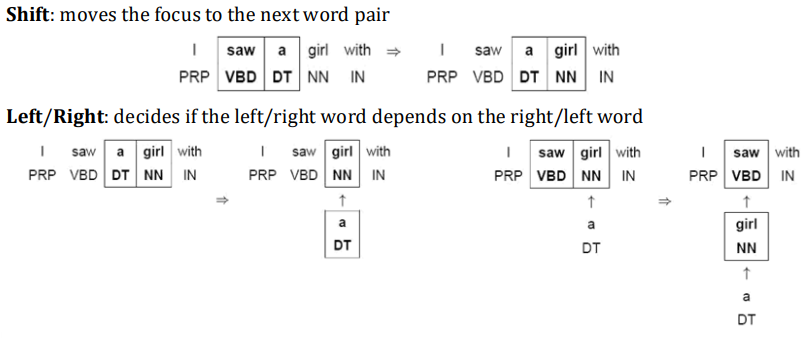
\includegraphics[width = 0.8\textwidth]{figs/transition.png}
\end{figure}

Se basa en un enfoque basado en pilas denominado «análisis sintáctico shift-reduce», desarrollado originalmente para analizar lenguajes de programación. Lo complicado del parseo no es construir la pila y el buffer, si no construir el oráculo o parser para que indique si dos palabras tienen dependencia para sacarlas de la pila y guardar la dependencia. 

\begin{figure}[h]
\centering
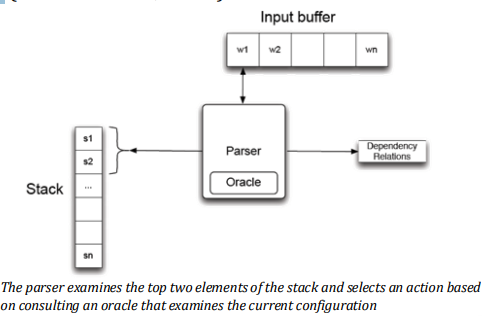
\includegraphics[width = 0.5\textwidth]{figs/transition-parser.png}
\end{figure}

El oráculo se crea con un algoritmo de aprendizaje automático o entrenando con un corpus. Así se van aplicando las relaciones encontradas.

\begin{figure}[h]
\centering
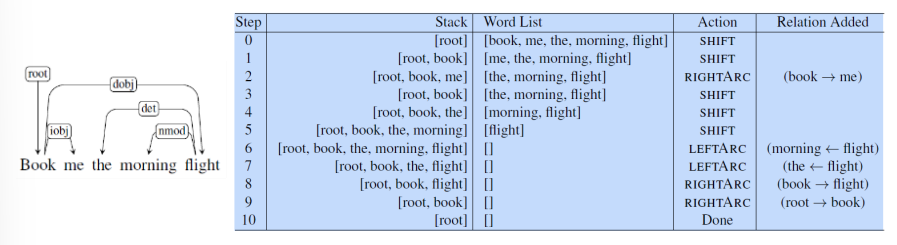
\includegraphics[width = \textwidth]{figs/transition-ej.png}
\end{figure}

\subsection{Parseo basado en grafos de dependencias}
Los \textbf{parseos basados en grafos} construyen un grafo completo con nodos dirigidos y con peso para encontrar el score más alta. Esta búsqueda es exhaustiva y encuentra el óptimo global. No importa si el grafo es proyectivo o no, pero el coste es de $O(n^3)$.

Se busca para maximizar las relaciones de dependencia con una métrica de score oportuna para la implementación. Entre las múltiples aproximaciones, está el \textbf{algoritmo de Chu-Liu-Edmond} que parte de una serie de premisas como grafo conexo, con peso y dirigido. Se pueden crear grafos más complejos con muchas relaciones de las que hay que decidir con cuál quedarnos.

\section{Evaluación de parsers}
Hay métricas a nivel de corpus y a nivel de oración. Hay métricas que ayudan a evaluar cuán bien funciona el parser, pero tampoco vamos a entrar en más detalle.

En resumen: tenemos el PoS tagging donde etiquetamos, el análisis de constituyentes y análisis de dependencias. Para cada uno de ellos necesitamos un corpus para entrenar y poder hacer el análisis posterior. Para cada análisis hay métricas que permiten evaluar el funcionamiento. PoS tagging es la entrada a los otros dos análisis. 